\documentclass[aspectratio=169,11pt]{beamer}

\usepackage[T1]{fontenc}
\usepackage[utf8]{inputenc}
\usepackage[british]{babel}
\usepackage{amssymb,amsmath,mathtools}
\usepackage{booktabs}
\usepackage{graphicx}

\usetheme{Madrid}
\useoutertheme{miniframes}
\setbeamertemplate{navigation symbols}{}

\graphicspath{{docs/apresentacao/apresentacao-assets/}{apresentacao-assets/}}

\newcommand{\R}{\mathbb{R}}
\newcommand{\Gtwo}{\mathrm{G}_2}
\newcommand{\SO}{\mathrm{SO}}
\newcommand{\Sym}{\operatorname{Sym}}

\title[Learning the metric of a \texorpdfstring{$\Gtwo$}{G2}-structure]
{\texorpdfstring{Learning the metric induced by a $\Gtwo$-structure}
{Learning the metric induced by a G2-structure}}
\subtitle{Generalisation and equivariance through data augmentation}
\author[Eduardo Toffolo]{Eduardo Toffolo}
\institute[Unicamp]{University of Campinas}
\date{MM845 --- AI for Geometry}

\begin{document}

% 0:25
\begin{frame}
    \titlepage
\end{frame}

\section{Problem}

% 0:55
\begin{frame}{Research question}
    \small
    A positive $3$-form $\varphi$ on an oriented $7$-dimensional vector space
    determines a unique metric $g_\varphi$.

    \vspace{-0.10cm}
    \begin{equation*}
        \varphi_0=e^{123}+e^{145}+e^{167}+e^{246}
        -e^{257}-e^{347}-e^{356}.
    \end{equation*}

    \begin{block}{Supervised task}
        Learn, from the $35$ coefficients of $\varphi$, the map
        \begin{equation*}
            F:\mathcal P\subset\Lambda^3(\R^7)^*
            \longrightarrow \Sym^+(7),
            \qquad F(\varphi)=g_\varphi,
        \end{equation*}
        whose output has $28$ independent entries.
    \end{block}

    \begin{alertblock}{Experimental question}
        Can a generic neural network approximate this map? Does rotation augmentation
        improve accuracy, generalisation and compatibility with the geometry?
    \end{alertblock}
\end{frame}

% 1:00
\begin{frame}{The exact formula and geometric identities}
    \begin{columns}[T,onlytextwidth]
        \column{0.49\textwidth}
        \begin{block}{Metric determined by $\varphi$}
            In an oriented basis with reference volume $\mathrm{vol}_0$,
            \begin{align*}
                (B_\varphi)_{ij}\,\mathrm{vol}_0
                &=\frac{1}{6}(\iota_{e_i}\varphi)\wedge
                  (\iota_{e_j}\varphi)\wedge\varphi,\\
                g_\varphi&=(\det B_\varphi)^{-1/9}B_\varphi.
            \end{align*}
        \end{block}

        If $\varphi=A^*\varphi_0$, then
        \begin{equation*}
            \boxed{g_\varphi=A^{\mathsf T}A}.
        \end{equation*}

        \column{0.48\textwidth}
        \begin{block}{Naturality}
            For $C\in\mathrm{GL}^+(7)$,
            \begin{equation*}
                F(C^*\varphi)=C^{\mathsf T}F(\varphi)C.
            \end{equation*}
        \end{block}

        \begin{block}{Homogeneity}
            For $t>0$,
            \begin{equation*}
                F(t\varphi)=t^{2/3}F(\varphi).
            \end{equation*}
        \end{block}

        These identities provide separate tests of equivariance and scaling.
    \end{columns}

    \vfill
    {\tiny Mathematical references: Karigiannis (2020) and Grigorian (2016).}
\end{frame}

\section{Data and methods}

% 1:00
\begin{frame}{Synthetic data and experimental protocol}
    \footnotesize
    \begin{columns}[T,onlytextwidth]
        \column{0.49\textwidth}
        \begin{block}{Exact-label generation}
            \begin{align*}
                A&=Q_1\operatorname{diag}(e^{s_1},\ldots,e^{s_7})Q_2,\\[-0.25em]
                \varphi&=A^*\varphi_0,\qquad g=A^{\mathsf T}A,
            \end{align*}
            with independent Haar $Q_1,Q_2\in\SO(7)$.

            \begin{itemize}
                \setlength{\itemsep}{1pt}
                \item ID: 30,000 sources, $s_i\in[-0.35,0.35]$;
                \item OOD: 4,500 sources, $s_i\in[-0.7,0.7]$, with at least one $|s_i|>0.35$.
            \end{itemize}
        \end{block}

        \column{0.48\textwidth}
        \begin{block}{Training and evaluation}
            \begin{itemize}
                \setlength{\itemsep}{1pt}
                \item ID split: 21,000 / 4,500 / 4,500;
                \item training subsets: 2,100, 7,000 and 21,000;
                \item seeds 11, 22 and 33: 27 fitted models;
                \item relative Frobenius error on ID and OOD;
                \item $\SO(7)$, $\mathrm{GL}^+(7)$, scaling and positivity tests.
            \end{itemize}
        \end{block}
    \end{columns}

    \vspace{-0.05cm}
    \begin{alertblock}{Reference check}
        The two exact formulas agree within $6\times10^{-16}$;
        the split precedes augmentation.
    \end{alertblock}
\end{frame}

% 1:05
\begin{frame}{Three models under the same protocol}
    \small
    The training objective is the mean squared relative Frobenius error:
    \begin{equation*}
        \mathcal L(\theta)=\frac{1}{N}\sum_{n=1}^N
        \frac{\|\widehat g_\theta(\varphi_n)-g_n\|_F^2}{\|g_n\|_F^2}.
    \end{equation*}

    \begin{columns}[T,onlytextwidth]
        \column{0.32\textwidth}
        \begin{block}{Ridge}
            \scriptsize Affine map from 35 coefficients to 28 symmetric entries.
            Positive definiteness is not guaranteed.
        \end{block}

        \column{0.32\textwidth}
        \begin{block}{MLP}
            \scriptsize Architecture $35\to128\to128\to28$, with ReLU and Adam.
            The output forms a triangular $L$, with a softplus diagonal, and
            $\widehat g=LL^{\mathsf T}$.
        \end{block}

        \column{0.32\textwidth}
        \begin{block}{MLP + rotations}
            \scriptsize Same network. At each epoch and for each source,
            \begin{equation*}
                (\varphi,g)\mapsto(C^*\varphi,C^{\mathsf T}gC),
            \end{equation*}
            with a new $C\in\SO(7)$.
        \end{block}
    \end{columns}

    \vspace{-0.18cm}
    \begin{alertblock}{Controlled comparison}
        \footnotesize Same sources, initialisation and minibatches: augmentation changes the views
        but retains 21,000 examples per epoch.
    \end{alertblock}
\end{frame}

\section{Results}

% 1:15
\begin{frame}{Accuracy: more data help, but the error remains high}
    \begin{center}
        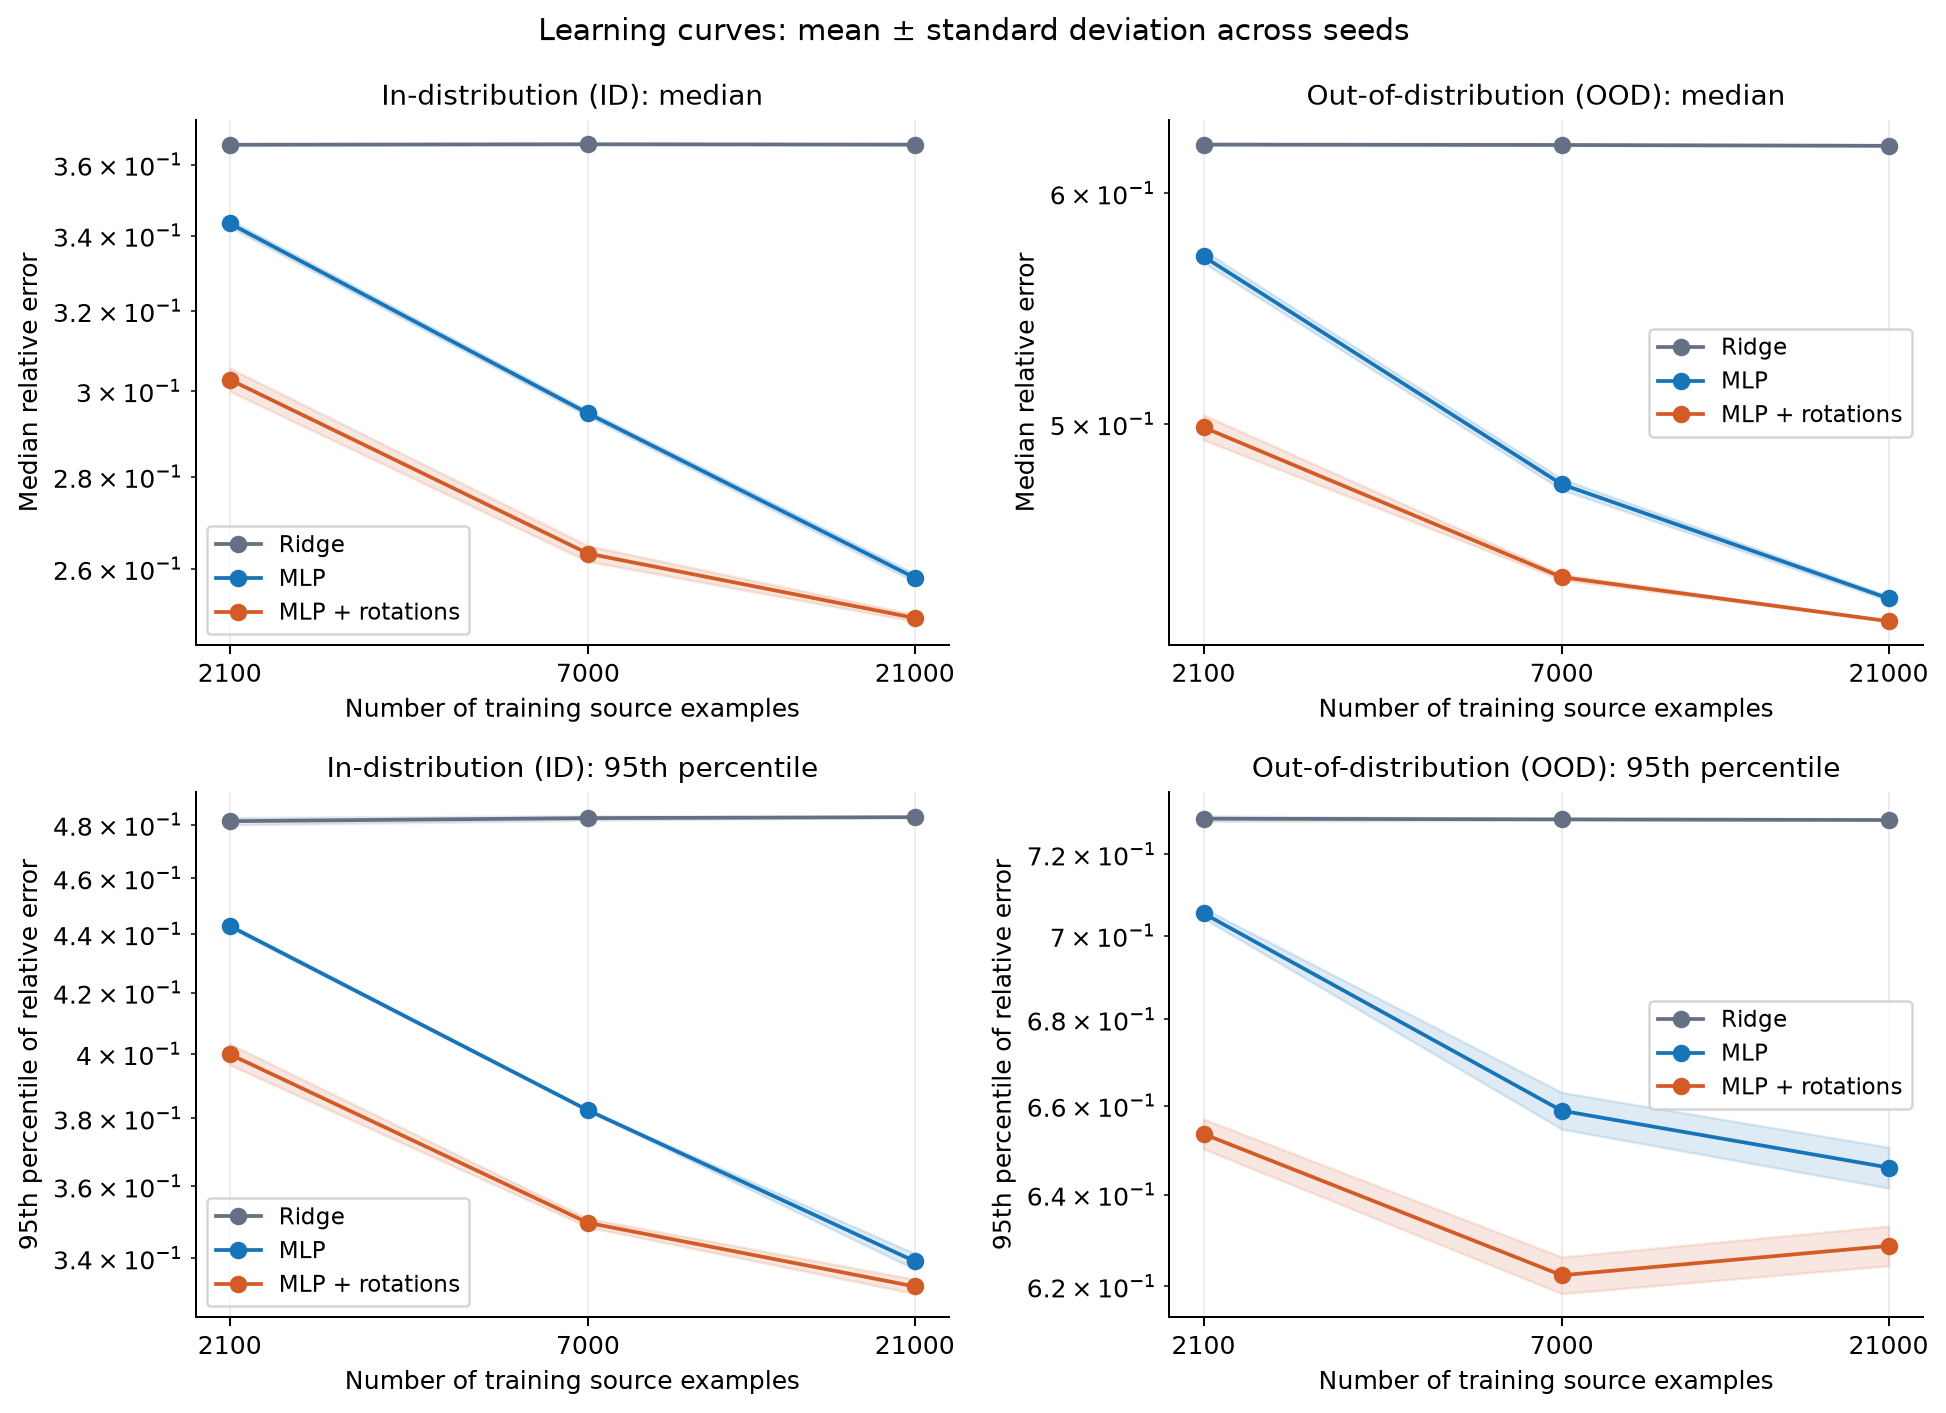
\includegraphics[width=0.70\textwidth,trim=0 270bp 0 0,clip]
        {learning_curves.png}
    \end{center}

    \vspace{-0.15cm}
    \begin{center}
        \scriptsize
        \begin{tabular}{lccc}
            \toprule
            & \textbf{Ridge} & \textbf{MLP} & \textbf{MLP + rotations} \\
            \midrule
            ID  & 36.58\% & 25.81\% & \textbf{24.99\%} \\
            OOD & 62.29\% & 43.57\% & \textbf{42.79\%} \\
            \bottomrule
        \end{tabular}
    \end{center}

    \scriptsize\textbf{Interpretation.}
    For 21,000 sources, these are means across three seed-level medians.
    The MLP outperforms ridge and augmentation helps modestly; the ID--OOD gap remains large.
\end{frame}

% 1:15
\begin{frame}{Equivariance: a modest improvement and a pitfall}
    \begin{center}
        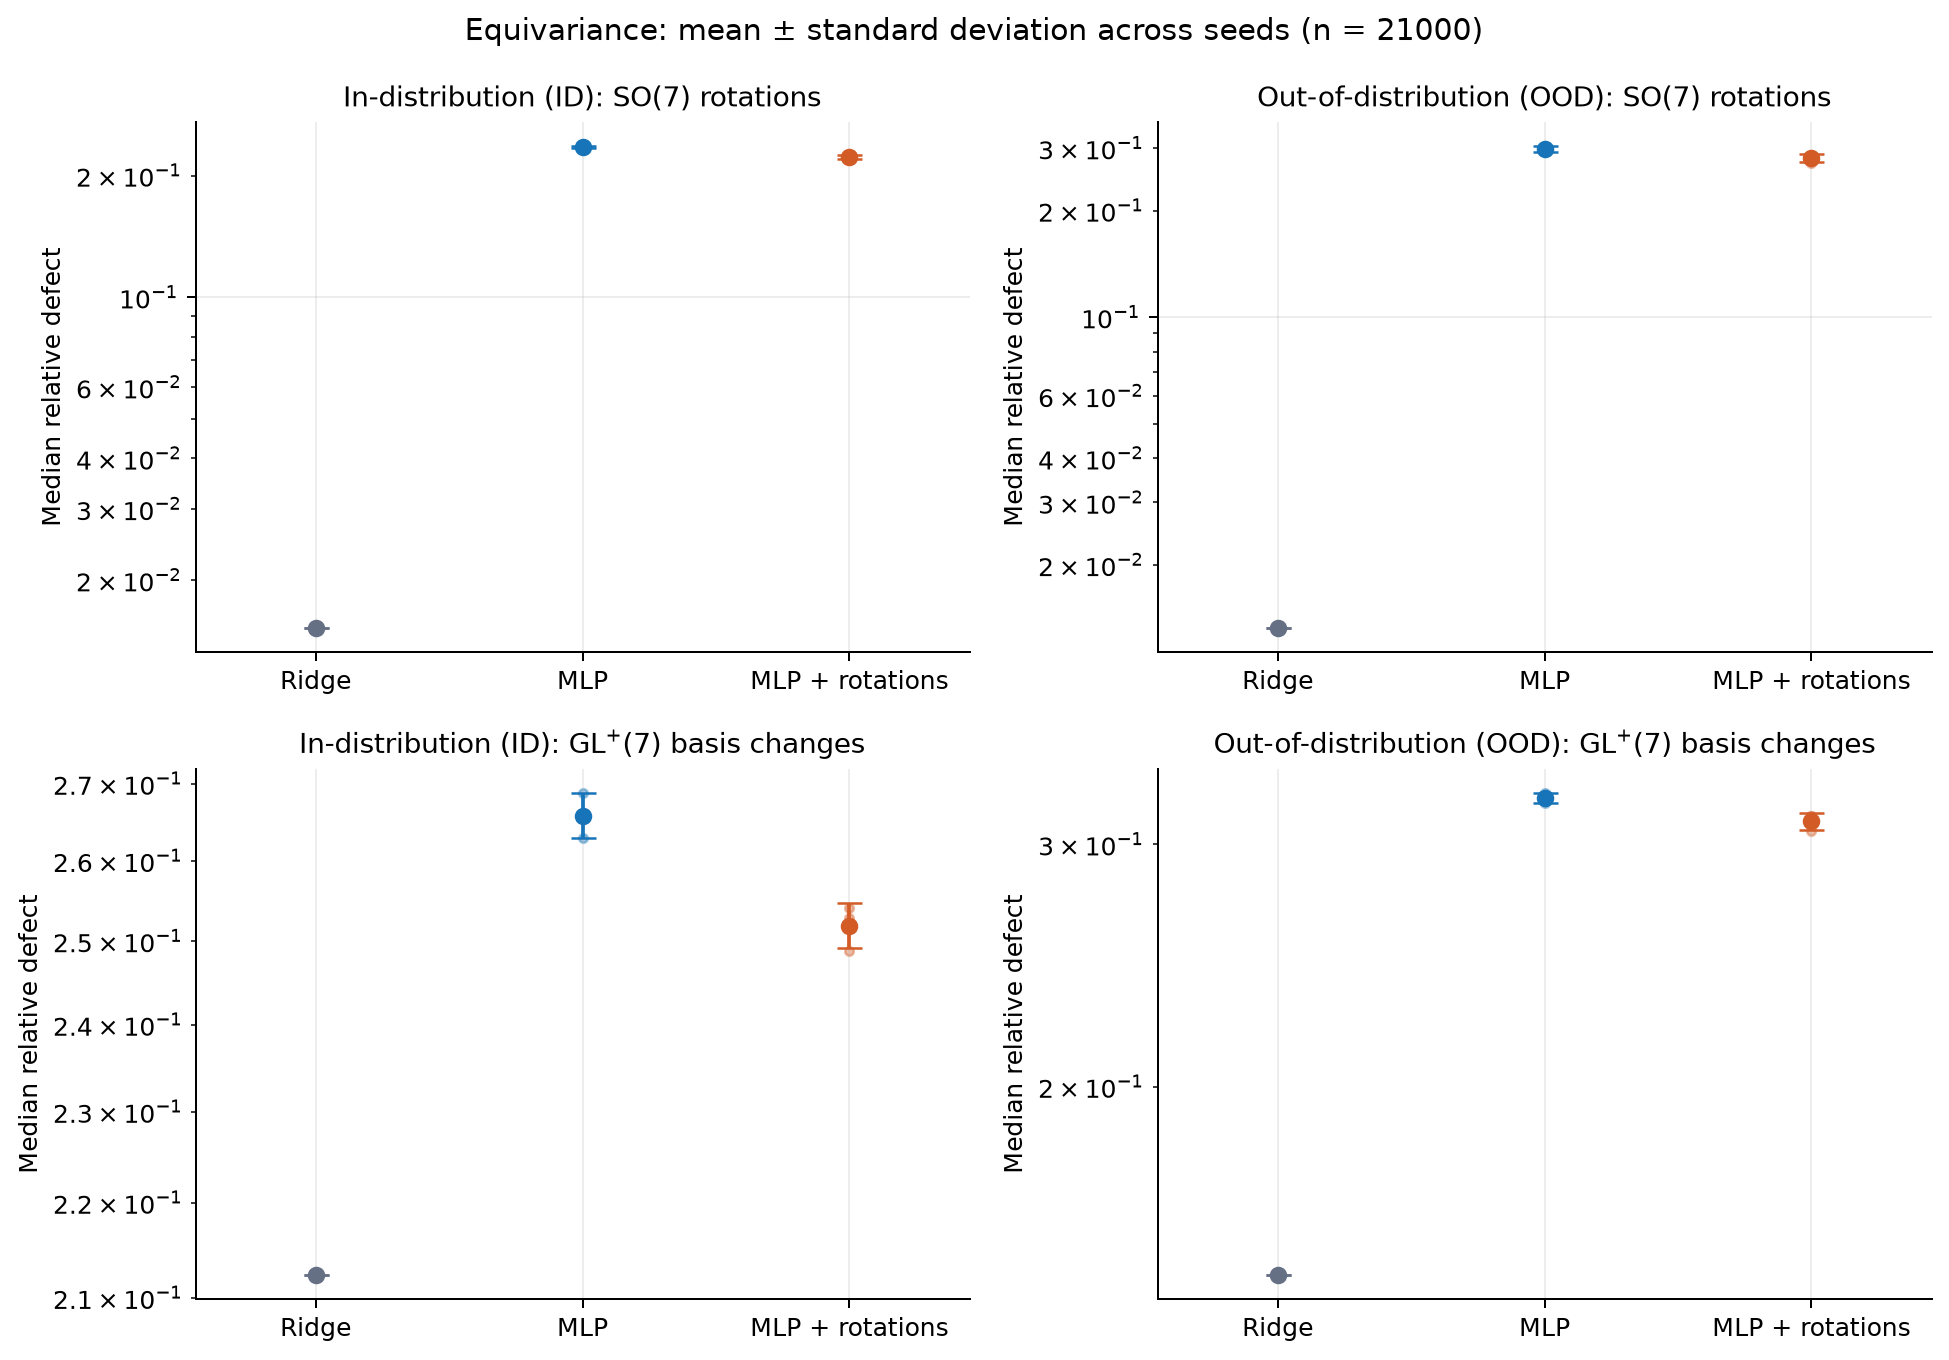
\includegraphics[width=0.70\textwidth,trim=0 260bp 0 0,clip]
        {equivariance.png}
    \end{center}

    \vspace{-0.10cm}
    \begin{columns}[T,onlytextwidth]
        \column{0.49\textwidth}
        \begin{block}{Effect of augmentation}
            \footnotesize
            The median $\SO(7)$ defect falls from $0.2355$ to $0.2223$ on ID
            and from $0.2985$ to $0.2818$ on OOD: a relative reduction of about 5.6\%.
        \end{block}

        \column{0.48\textwidth}
        \begin{alertblock}{Why does ridge look better?}
            \footnotesize
            It almost always predicts $1.08288I$. An almost constant scalar output
            has a low rotation defect, yet can ignore the input and predict the wrong metric.
        \end{alertblock}
    \end{columns}
\end{frame}

% 1:00
\begin{frame}{Rotation augmentation does not learn the scaling law}
    \begin{center}
        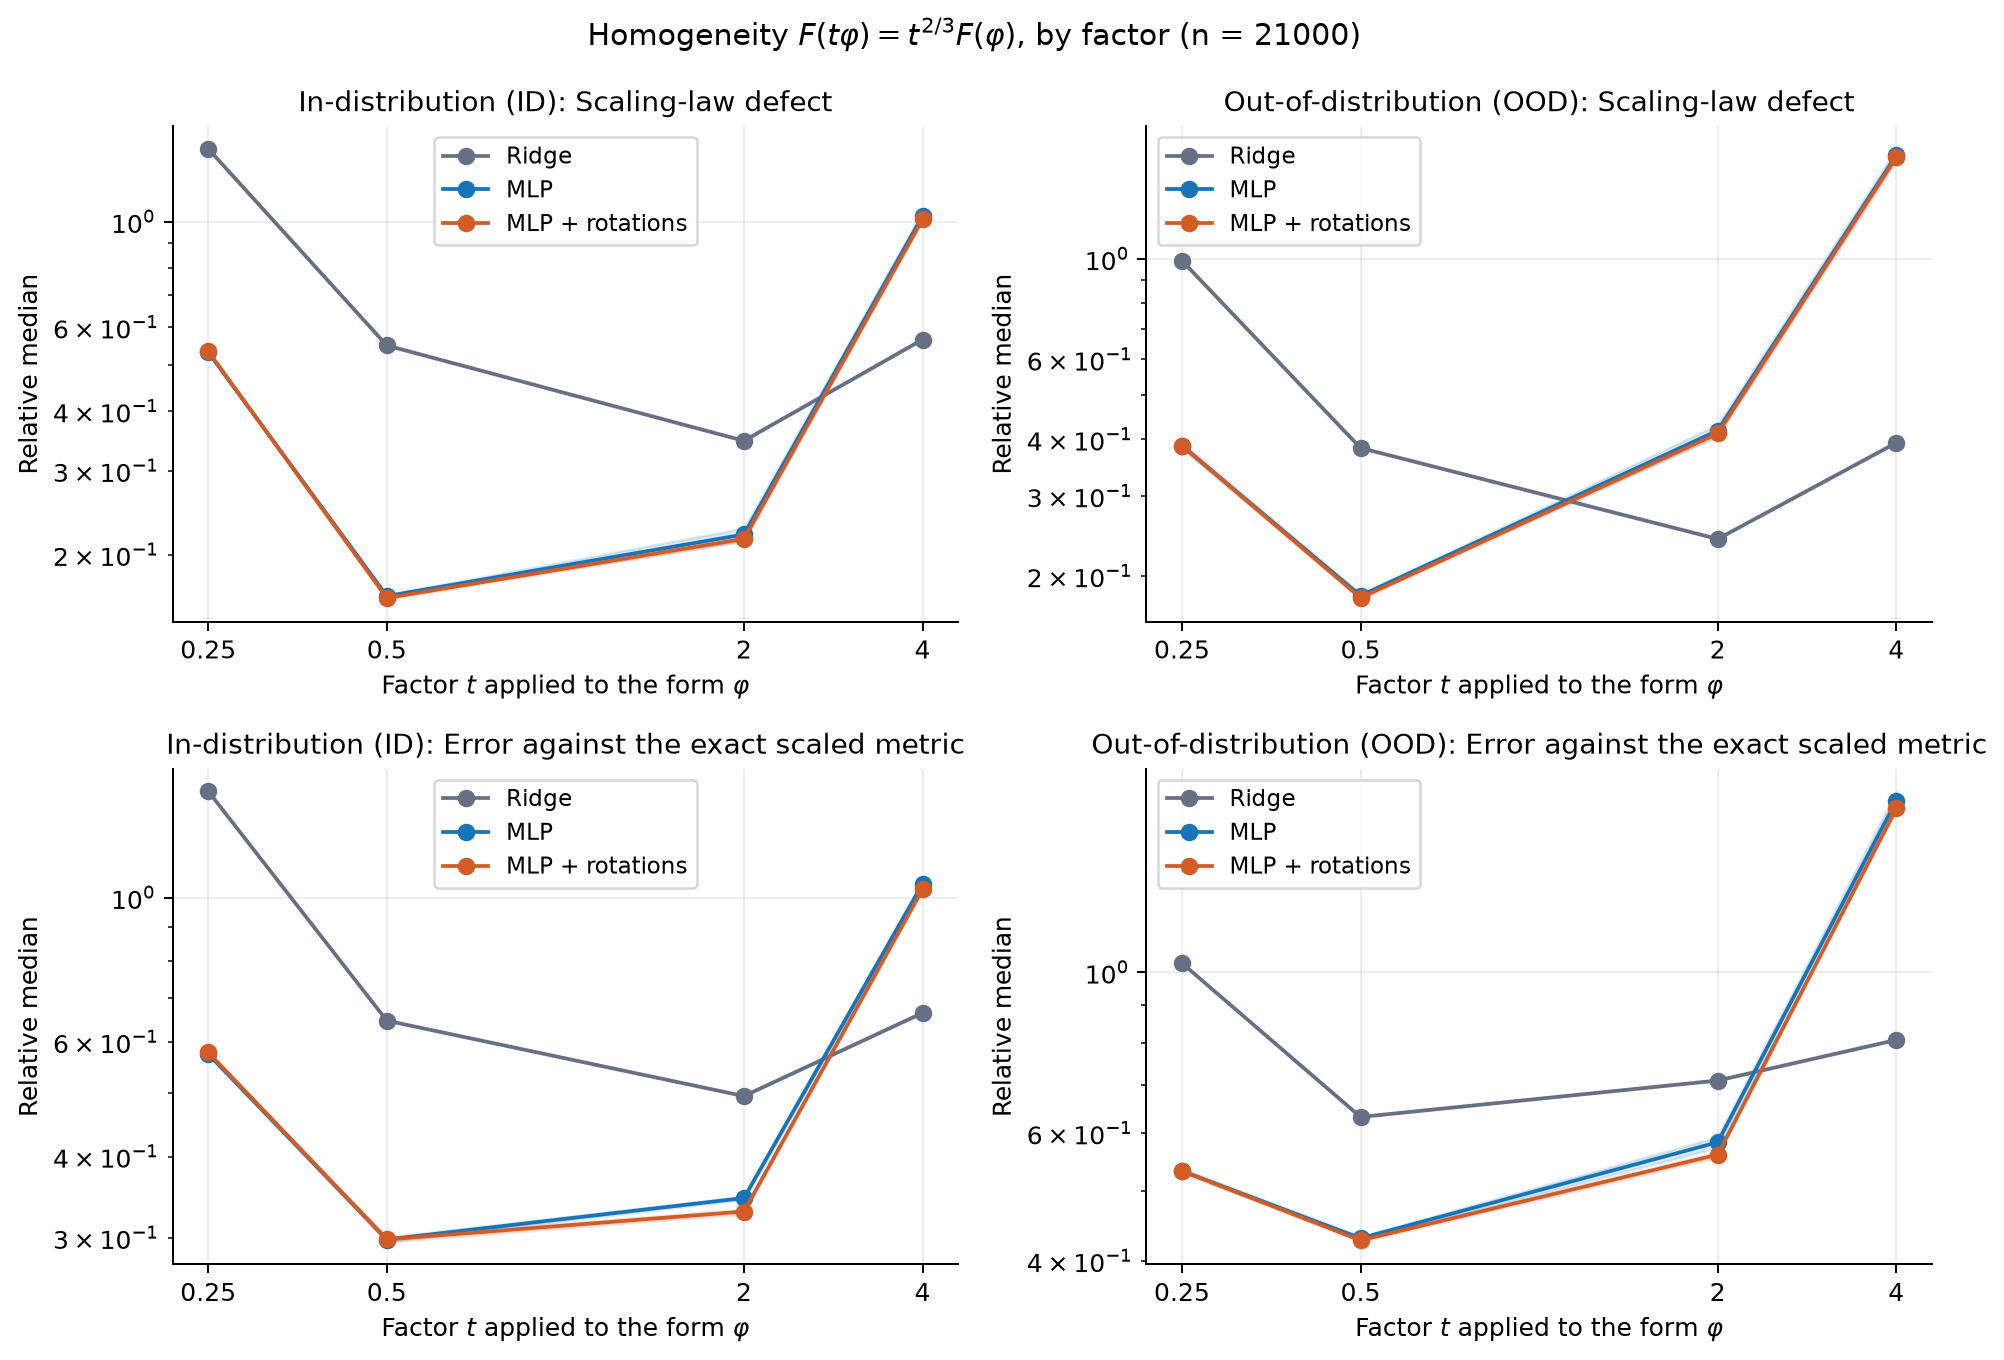
\includegraphics[width=0.70\textwidth,trim=0 260bp 0 0,clip]
        {scaling.png}
    \end{center}

    \begin{block}{Result}
        \footnotesize
        Augmentation by $\SO(7)$ does not enforce
        $\widehat F(t\varphi)=t^{2/3}\widehat F(\varphi)$.
        The defect grows for factors far from the training range, especially at $t=4$,
        on both ID and OOD. Accuracy, equivariance and homogeneity are distinct diagnostics.
    \end{block}
\end{frame}

% 1:05
\begin{frame}{Why is the error still large?}
    \small
    \begin{columns}[c,onlytextwidth]
        \column{0.47\textwidth}
        \begin{center}
            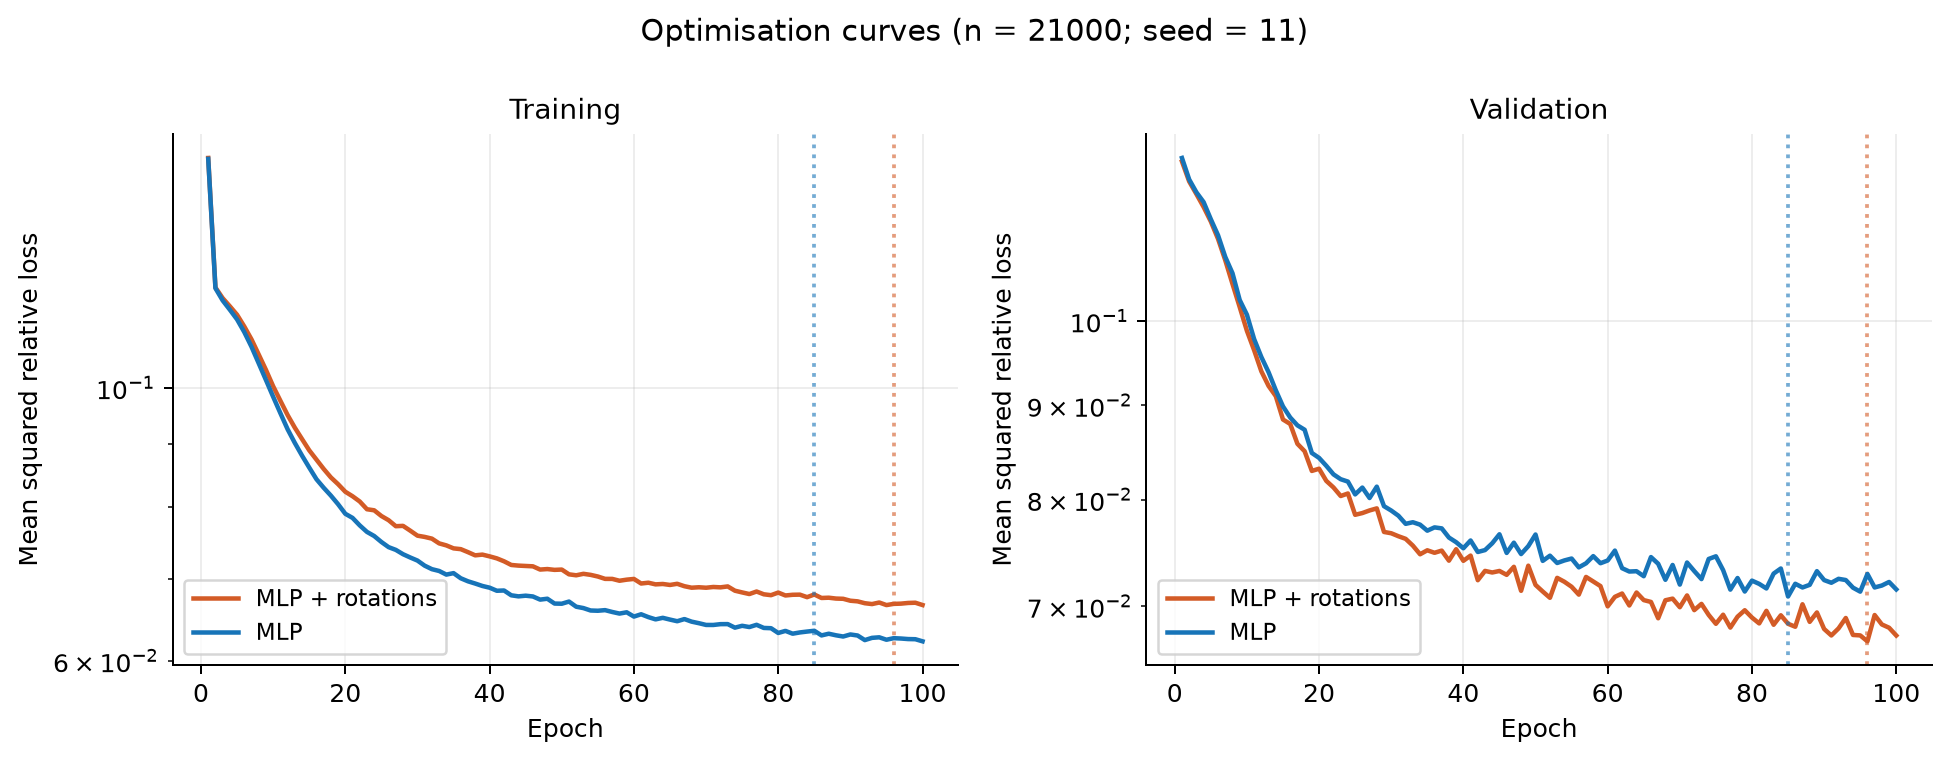
\includegraphics[width=\textwidth]{training_curves.png}
        \end{center}
        {\scriptsize Training and validation curves for $n=21{,}000$, seed 11.}

        \column{0.50\textwidth}
        \begin{block}{Hypotheses consistent with the results}
            \begin{itemize}\footnotesize
                \item cubic map with determinant normalisation;
                \item generic MLP with no built-in geometric identities;
                \item best checkpoints near 100 epochs; OOD increases scale and anisotropy.
            \end{itemize}
        \end{block}

        \begin{alertblock}{Next experiments}
            \footnotesize Test overfitting on a small sample; then increase capacity and budget,
            or impose homogeneity and equivariance.
        \end{alertblock}
    \end{columns}
\end{frame}

\section{Conclusion}

% 0:55
\begin{frame}{Conclusions}
    \begin{enumerate}
        \item Synthetic generation provides exact labels and supports controlled tests of geometric properties.
        \item The MLP clearly reduces the error relative to ridge; rotation augmentation improves accuracy and the $\SO(7)$ defect for every seed, but only modestly.
        \item Median errors of approximately 25\% on ID and 43\% on OOD do not constitute a high-accuracy approximation.
        \item The network does not automatically learn exact equivariance or the scaling law. The geometric formula remains the reference.
    \end{enumerate}

    \begin{alertblock}{Answer to the experimental question}
        Data augmentation helps consistently under this protocol, but it does not replace
        an architecture that incorporates the mathematical structure of the problem.
    \end{alertblock}

    \vfill
    {\tiny Results are reproducible across three seeds; hyperparameters and checkpoints were selected on validation data.}
\end{frame}

\begin{frame}[noframenumbering]
    \centering
    \Huge Thank you

    \vspace{0.8cm}
    \Large Questions?
\end{frame}

\end{document}
